%   % !TEX root = ../../VIII,3_Rahmen-TeX_8-1.tex
%
%
%   Band VIII, 3 N.~??S01.12
%   Signatur/Tex-Datei: LH_37_05_090-091
%   RK-Nr. 57264
%   \ref{dcc_10}
%   Überschrift: De corporum concursus scheda decima
%   Modul: Mechanik / Stoß ( )
%   Datierung: Januar 1678
%   WZ: (Bl. 91) LEd-WZ 803017 = RK-WZ 1264 (insgesamt: eins)
%   SZ:   (keins)
%   Bilddateien (PDF): 
%      LH_37_05_090-091_d1 ((ex: lh37,5,90r))
%      LH_37_05_090-091_d2 ((ex: lh37,5,90v-1))
%      LH_37_05_090-091_d3 ((ex: lh37,5,90v-2))
%      LH_37_05_090-091_d4 ((ex: lh37,5,90v-3))
%      LH_37_05_090-091_d5 ((ex: lh37,5,91v-1))
%      LH_37_05_090-091_d6 ((ex: lh37,5,91v-2))
%      (insgesamt: sechs)
%   Verzeichniseinträge: vollständig
%   \textls{} statt \textso{} (Ausnahme: Personenverzeichnis)
%
%
\selectlanguage{ngerman}%
\frenchspacing%
%
\begin{ledgroupsized}[r]{120mm}%
\footnotesize%
\pstart%
\noindent%
\textbf{Überlieferung:}%
\pend%
\end{ledgroupsized}%
\begin{ledgroupsized}[r]{114mm}%
\footnotesize%
\pstart%
\parindent -6mm%
\makebox[6mm][l]{\textit{L}}%
Konzept:
LH XXXVII~5, Bl.~90\textendash91.
Zwei Blatt 2\textsuperscript{o},
die wohl ursprünglich einen Bogen bildeten;
ein Wasserzeichen auf Bl.~91;
Papiererhaltungsmaßnahmen.
Zweieinhalb vollbeschriebene Seiten auf Bl.~90~r\textsuperscript{o}, 90~v\textsuperscript{o} und 91~v\textsuperscript{o},
die den Text von N.~\ref{dcc_09} %??S01\textsubscript{11} 
fortsetzen.
Bl.~91~r\textsuperscript{o} überliefert einen gestrichenen Abschnitt von N.~\ref{dcc_06-2} %??S01\textsubscript{8}
(S.~\pageref{LH_37_05_091r_gestrtab}\textendash\pageref{LH_37_05_091r_ende}).
\pend%
\end{ledgroupsized}%
%
\begin{ledgroupsized}[r]{114mm}%
\footnotesize%
\pstart%
\parindent -6mm%
\makebox[6mm][l]{\textit{E}}%
\textsc{Fichant} 1994, S.~166\textendash171
(mit kommentierter französischer Übersetzung, S.~331\textendash337).%
\cite{01056}%
\pend%
\end{ledgroupsized}%
%
\selectlanguage{latin}%
\frenchspacing%
%
%
\vspace{8mm}
\count\Bfootins=1000%
\count\Afootins=1200%
\count\Cfootins=1000
\normalsize%
\pstart%
\noindent%
%
\lbrack 90~r\textsuperscript{o}\rbrack% \ %%%%    Blatt 90r
\hspace{39mm}
De concursu corporum%
\protect\index{Sachverzeichnis}{concursus corporum}
\hspace{16mm}
Januar. 1678 et febr.%
\pend%
\pstart%
\noindent%
\centering%
Scheda decima%
\protect\index{Sachverzeichnis}{scheda}
\pend%
\vspace{0,5em}%
%
\pstart%
\noindent%
Postquam%
\edlabel{LH_37_05_090r_satisfecimus-1}
 in praecedentibus schedis%
\protect\index{Sachverzeichnis}{scheda}
inprimis
%
\edtext{octava et nona}{%
\lemma{octava et nona}\Cfootnote{%
N.~\ref{dcc_08} und N.~\ref{dcc_09}.% ??S01\textsubscript{10} und N.~??S01\textsubscript{11}.% 
}}
%
solida demonstratione nobis satisfecimus,%
\protect\index{Sachverzeichnis}{demonstratio solida}%
\edlabel{LH_37_05_090r_satisfecimus-2}
ostendendo
quod
eadem manente vi%
\protect\index{Sachverzeichnis}{vis manens eadem}
necessario etiam eadem maneat via centri gravitatis;%
\protect\index{Sachverzeichnis}{via centri gravitatis eadem}%
\protect\index{Sachverzeichnis}{centrum gravitatis}
unde etiam eandem distantiam manere colligitur,%
\protect\index{Sachverzeichnis}{distantia corporum eadem}
quando corpora vim ictu acceptam perfecte reddunt.%
\protect\index{Sachverzeichnis}{vis ictu accepta}%
\protect\index{Sachverzeichnis}{vis perfecte reddita}%
\protect\index{Sachverzeichnis}{corpus vim reddens}
Hinc cogitandum esset
quid fiat,
quando unum corpus incurrit in plura,%
\protect\index{Sachverzeichnis}{corpus in plura incurrens}
et plura in unum;%
\protect\index{Sachverzeichnis}{corpora in unum incurrentia}
tunc enim non aeque determinata sunt omnia ex his duabus
%
\edtext{regulis,%
\protect\index{Sachverzeichnis}{regulae de concursu corporum}
ubi variae tamen ex ratione constitui poterunt aequationes,%
\protect\index{Sachverzeichnis}{aequatio}
ut quarum eadem ratio%
\protect\index{Sachverzeichnis}{ratio eadem}
eodem modo tractentur.
Agendum et de obliquis percussionibus,%
\protect\index{Sachverzeichnis}{percussio obliqua}}{%
\lemma{regulis}\Bfootnote{%
\textit{(1)}~. Verum quaerendum item de percussionibus obliquis.
\textit{(2)}~, ubi ante \textlangle\textendash\textrangle\
\textit{(3)}~, ubi variae \lbrack...\rbrack\ ut quarum
\textit{(a)}~eaedem
\textit{(b)}~eadem ratio, \lbrack...\rbrack\ obliquis percussionibus,%
~\textit{L}}}
%
ubi nova et subtilissima inquisitio,%
\protect\index{Sachverzeichnis}{inquisitio subtilissima}
utrum corpus pelli an%
\protect\index{Sachverzeichnis}{corpus pulsum}
circa centrum agi malit.%
\protect\index{Sachverzeichnis}{corpus circa centrum actum}
Veniendum et ad percussiones obliquas,%
\protect\index{Sachverzeichnis}{percussio obliqua}
item ad concursum corporum solidorum et liquidorum,%
\protect\index{Sachverzeichnis}{concursus corporum solidorum et liquidorum}%
\protect\index{Sachverzeichnis}{corpora solida et liquida concurrentia}%
\protect\index{Sachverzeichnis}{corpus solidum}%
\protect\index{Sachverzeichnis}{corpus liquidum}
item duorum liquidorum simul,%
\protect\index{Sachverzeichnis}{concursus corporum liquidorum}%
\protect\index{Sachverzeichnis}{corpora liquida concurrentia}%
\protect\index{Sachverzeichnis}{corpus liquidum}
ut venti et aquae,%
\protect\index{Sachverzeichnis}{concursus venti et aquae}%
\protect\index{Sachverzeichnis}{ventus cum aqua concurrens}%
\protect\index{Sachverzeichnis}{aqua cum vento concurrens}
item de vi Elateriorum.%
\protect\index{Sachverzeichnis}{vis elaterii}%
\protect\index{Sachverzeichnis}{elaterium}
Item de vi quae perditur frictione,%
\protect\index{Sachverzeichnis}{vis frictione perdita}%
\protect\index{Sachverzeichnis}{frictio}
in quibus omnibus utilissimae poterunt esse considerationes de servata vi,%
\protect\index{Sachverzeichnis}{consideratio de vi servata}%
\protect\index{Sachverzeichnis}{vis servata}
%
\edtext{et de directione}{%
\lemma{et}\Bfootnote{%
\hspace{-0,5mm}de
\textit{(1)}~via
\textit{(2)}~directione%
~\textit{L}}}
%
centri gravitatis.%
\protect\index{Sachverzeichnis}{directio centri gravitatis}%
\protect\index{Sachverzeichnis}{consideratio de directione centri gravitatis}
Huc
%
\edtext{pertinet et inquisitio}{%
\lemma{pertinet}\Bfootnote{%
\hspace{-0,5mm}et
\textit{(1)}~ducti
\textit{(2)}~inquisitio%
~\textit{L}}}
%
de motu projectorum,%
\protect\index{Sachverzeichnis}{inquisitio de motu projectorum}%
\protect\index{Sachverzeichnis}{motus projectorum}
deque aeris resistentia,%
\protect\index{Sachverzeichnis}{inquisitio de resistentia aeris}%
\protect\index{Sachverzeichnis}{resistentia aeris}
quam perfecte determinari posse arbitror.
Utamur semper hac via de motu perpetuo efficiendo,%
\protect\index{Sachverzeichnis}{motus perpetuus artificialis}%
\protect\index{Sachverzeichnis}{via de motu perpetuo efficiendo}
et semper pulchra theoremata detegemus.%
\protect\index{Sachverzeichnis}{theorema pulchrum}%
\pend%
%
\pstart%
Ponamus corpus unum in alia duo impingere,%
\protect\index{Sachverzeichnis}{corpus in duo impingens}
eodemque modo se ad
%
\edtext{illa duo habere,}{%
\lemma{illa}\Bfootnote{%
\textit{(1)}~habere
\textit{(2)}~duo habere,%
~\textit{L}}}
%
seu ea duo similiter ad ipsum esse posita,
quaerimus tres incognitas,%
\protect\index{Sachverzeichnis}{incognita quaesita}
scilicet
%
\edtext{corporum trium celeritates%
\protect\index{Sachverzeichnis}{celeritas post ictum}
dato tempore%
\protect\index{Sachverzeichnis}{tempus datum post ictum}
post ictum,%
\protect\index{Sachverzeichnis}{ictus trium corporum}
sed praeterea et angulos duorum,%
\protect\index{Sachverzeichnis}{angulus corporis excipientis}%
}{%
\lemma{corporum}\Bfootnote{%
\textit{(1)}~\textbar~trium \textit{erg.}~\textbar\ celeritates post ictum
\textit{(2)}~trium
\textit{(a)}~loca
\textit{(b)}~celeritates dato tempore post ictum,
\textit{(aa)}~et
\textit{(bb)}~sed praeterea et
\textit{(aaa)}~angulos; habemus
\textit{(bbb)}~angulos duorum,%
~\textit{L}}}
%
quorum \makebox[1.0\textwidth][s]{unus ut alius;
sunt ergo quatuor incognitae,%
\protect\index{Sachverzeichnis}{incognita quaesita}
imo revera tres tantum,
quia celeritas unius}
\pend
\newpage
 % Diagramm Fig.~1
  \centerline{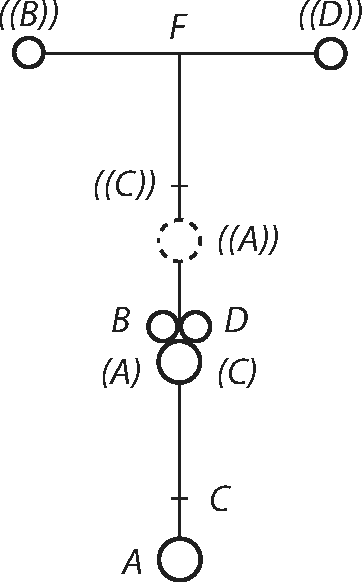
\includegraphics[width=0.27\textwidth]{gesamttex/edit_VIII,3/images/LH_37_05_090-091_d1.pdf}}%
  \vspace{0.5em}
  \centerline{\lbrack\textit{Fig.~1}\rbrack}%
%  \label{LH_37_05_090r_Fig.1}%
  \vspace{1.5em}%
\pstart
\noindent excipientium
quae alterius;%
\protect\index{Sachverzeichnis}{celeritas corporis excipientis}%
\protect\index{Sachverzeichnis}{corpora excipientia duo}
quaeritur ergo celeritas incurrentis simplicis,%
\protect\index{Sachverzeichnis}{celeritas corporis incurrentis}%
\protect\index{Sachverzeichnis}{corpus impingens simplex}
celeritas unius excipientis,%
\protect\index{Sachverzeichnis}{celeritas corporis excipientis}
et angulus unius excipientis,%
\protect\index{Sachverzeichnis}{angulus corporis excipientis}
quae sunt tria ignota.%
\protect\index{Sachverzeichnis}{ignotum}
Sunt
%
\edtext{vero duae}{%
\lemma{vero}\Bfootnote{%
\textit{(1)}~tres
\textit{(2)}~duae%
~\textit{L}}}
%
tantum aequationes:%
\protect\index{Sachverzeichnis}{aequatio}
aequalitas virium,%
\protect\index{Sachverzeichnis}{aequalitas virium corporum concurrentium}
%
\edtext{et aequalis celeritas}{%
\lemma{et}\Bfootnote{%
\textit{(1)}~aequalitas
\textit{(2)}~processus
\textit{(3)}~aequalis celeritas%
~\textit{L}}}
%
centri gravitatis.%
\protect\index{Sachverzeichnis}{aequalitas celeritatis centri gravitatis}
Imo datur non
%
\edtext{tantum centri gravitatis celeritatis aequalitas,}{%
\lemma{tantum}\Bfootnote{%
\textit{(1)}~aequalitas
\textit{(2)}~centri gravitatis celeritatis aequalitas,%
~\textit{L}}}
%
sed et datur ejus angulus,%
\protect\index{Sachverzeichnis}{angulus centri gravitatis}
seu locus.%
\protect\index{Sachverzeichnis}{locus centri gravitatis}
Hinc puto plus aliquid duci posse.
\pend%
%
\pstart%
(\protect\vphantom)%
Tota natura est irresistibilis.%
\protect\index{Sachverzeichnis}{natura irresistibilis}
Hinc et vires eaedem servantur,%
\protect\index{Sachverzeichnis}{vis corporum concurrentium servata}
et directio quoque.%
\protect\index{Sachverzeichnis}{directio centri gravitatis servata}%
\protect\vphantom()%
\pend%
%
\pstart%
Patet in hoc casu,
quia \textit{C(C)} aequ. \textit{(C)((C))},
duo tantum quaeri \textit{(A)((A))} et \textit{F((B))},
quia \textit{F((C))} datur ex data \textit{((A))((C))}
at \textit{((A))((C))} datur
ex data \textit{(A)((A))} et \textit{(C)((C))}.%
\pend%
%
\pstart%
Facillimum esse
paralogismos%
\protect\index{Sachverzeichnis}{paralogismus}
committere in hac materia
vel hinc patet,
%
\edtext{ostendimus vim aestimandam%
\protect\index{Sachverzeichnis}{vis aestimanda}
ex ductu corporis in quadratum celeritatis,%
\protect\index{Sachverzeichnis}{ductus corporis in quadratum celeritatis}%
}{%
\lemma{ostendimus \lbrack...\rbrack\ celeritatis}\Cfootnote{%
Vgl. N.~\ref{dcc_08}, % ??S01\textsubscript{10}
S.~\refpassage{LH_37_05_086r_reformatio_idzg-1}{LH_37_05_086r_reformatio_idzg-2}.
}}
%
hinc sequeretur%
\lbrack:\rbrack\
si duo corpora%
\protect\index{Sachverzeichnis}{corpora concurrentia}
quorum magnitudines reciproce%
\protect\index{Sachverzeichnis}{magnitudo corporum concurrentium}
ut quadrata celeritatum concurrerent,%
\protect\index{Sachverzeichnis}{quadratum celeritatis}
ea se esse mutuo repulsura,
quod tamen non fit;
ratio,
quia habent quidem eandem vim
%
\edtext{\lbrack accedendi\rbrack,%
\protect\index{Sachverzeichnis}{vis ascendendi}%
\protect\index{Sachverzeichnis}{vis discedendi}%
}{%
{\lemma{ascendendi}\Bfootnote{%
\textit{L~ändert Hrsg.}
}}%
{\lemma{\lbrack accedendi\rbrack}\Cfootnote{%
Siehe zu dieser Konjektur N.~\ref{dcc_09},
S.~\refpassage{LH_37_05_089v_accedendi-1}{LH_37_05_089v_accedendi-2}.%
}}}
%
sed aliud est de vi agendi in se invicem,%
\protect\index{Sachverzeichnis}{vis corporum agendi in se invicem}
seu sese propellendi.%
\protect\index{Sachverzeichnis}{vis corporis sese propellendi}
%
%
\lbrack90~v\textsuperscript{o}\rbrack\ %%%%    Blatt 90v
%
\pend%
\newpage%
%
\pstart%
%
\edtext{}{%
\lemma{\textit{Am Rand:}}\Afootnote{%
Percussio videtur esse secundum perpendicularem,%
\protect\index{Sachverzeichnis}{percussio secundum perpendicularem}
quia pone corpus \textit{B} incurrere oblique in chordam tensam \textit{AD}%
\protect\index{Sachverzeichnis}{corpus incurrens in chordam tensam}%
\protect\index{Sachverzeichnis}{chorda tensa}
eamque in curvam \textit{AED} flectere,%
\protect\index{Sachverzeichnis}{curva}%
\protect\index{Sachverzeichnis}{chorda flexa}
utique incursus obliquus \textit{FE}%
\protect\index{Sachverzeichnis}{incursus obliquus}
tantum flexit ac retendit chordam%
\protect\index{Sachverzeichnis}{chorda flexa}%
\protect\index{Sachverzeichnis}{chorda tensa}
quantum incursus rectus \textit{GE},%
\protect\index{Sachverzeichnis}{incursus rectus}
adeoque vis non nisi in perpendiculari aestimabitur.%
\protect\index{Sachverzeichnis}{vis in perpendiculari aestimanda}
Et idem erit effectus%
\protect\index{Sachverzeichnis}{effectus percussionis}
ac si corpus duplici motu ferretur,%
\protect\index{Sachverzeichnis}{corpus motu duplici latum}%
\protect\index{Sachverzeichnis}{motus duplex}
recto simul et parallelo.%
\protect\index{Sachverzeichnis}{motus rectus}%
\protect\index{Sachverzeichnis}{motus parallelus}%
\newline%
\newline%
%
%        Diagramm Fig.~2
  \centerline{\protect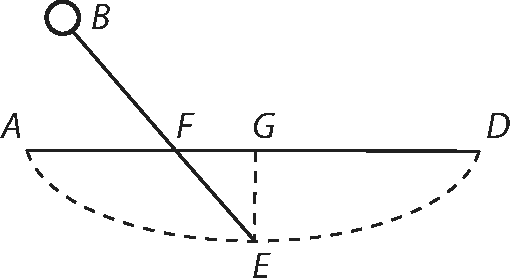
\includegraphics[width=0.39\textwidth]{gesamttex/edit_VIII,3/images/LH_37_05_090-091_d2.pdf}}%
  \vspace{0.5em}
  \centerline{\lbrack\textit{Fig.~2}\rbrack}%
%  \label{LH_37_05_090v_Fig.2}%
%
}}%
%
Hoc axioma:%
\protect\index{Sachverzeichnis}{axioma}%
\textls{ Naturam%
\protect\index{Sachverzeichnis}{natura irresistibilis}
totam esse irresistibilem }%
efficit tum ut vires maneant eaedem,%
\protect\index{Sachverzeichnis}{vis eadem manens}
tum ut eadem maneat directio centri gravitatis.%
\protect\index{Sachverzeichnis}{directio centri gravitatis}%
\protect\index{Sachverzeichnis}{centrum gravitatis}
Duo enim illa corpora
%
\edtext{vel plura}{%
\lemma{vel}\Bfootnote{%
\hspace{-0,5mm}plura
\textit{erg.~L}}}
%
de quibus agitur,
ponendo sola,
et
%
\edtext{ab}{%
\lemma{ab}\Bfootnote{%
\textit{erg.~L}}}
%
aliorum in ipsa actione%
\protect\index{Sachverzeichnis}{actio corporum}
animum abstrahendo,%
\protect\index{Sachverzeichnis}{animus}
ipsa totam naturam%
\protect\index{Sachverzeichnis}{natura tota}
seu quasi Mundum constituunt separatum.%
\protect\index{Sachverzeichnis}{mundus separatus}
Vires autem suas%
\protect\index{Sachverzeichnis}{vis machinae}
retinet haec machina tota,%
\protect\index{Sachverzeichnis}{machina tota}
quia nihil eas imminuit,%
\protect\index{Sachverzeichnis}{vis imminuta}
et directionem etiam%
\protect\index{Sachverzeichnis}{directio machinae}
%
\edtext{retinet in summa,%
\protect\index{Sachverzeichnis}{directio in summa retenta}
quatenus}{%
\lemma{retinet}\Bfootnote{\hspace{-0,5mm}%
\textit{(1)}~, quia
\textit{(2)}~in summa, quatenus%
~\textit{L}}}
%
omnia eandem in summa habent directionem.%
\pend%
%
\pstart%
Videndum
quid fiat in tota natura.%
\protect\index{Sachverzeichnis}{natura tota}
Imo in nostro systemate,%
\protect\index{Sachverzeichnis}{systema nostrum}
%
\edtext{propositio illa de incremento celeritatis perfecto%
\protect\index{Sachverzeichnis}{propositio de incremento celeritatis perfecto}%
\protect\index{Sachverzeichnis}{incrementum celeritatis perfectum}%
}{%
\lemma{propositio \lbrack...\rbrack\ perfecto}\Cfootnote{%
Anspielung nicht aufgelöst.%
%??? Wenn Leibniz hier auf den Impulserhalt anspielt, dann vgl. etwa N.~\ref{dcc_08}, S.~\refpassage{LH_37_05_087v_eskfz-1}{LH_37_05_087v_eskfz-2};
%N.~\ref{dcc_09}, \refpassage{LH_35_07_089v_tflk-1}{LH_35_07_089v_tflk-2}. ???%
}}
%
non potest esse rigorose vera.%
\protect\index{Sachverzeichnis}{propositio rigorose vera}
Praeterea an extra systema,%
\protect\index{Sachverzeichnis}{systema nostrum}
servanda est quantitas motus?%
\protect\index{Sachverzeichnis}{quantitas motus servanda}
An forte nihilominus fieri potest,
ut in toto Mundo%
\protect\index{Sachverzeichnis}{mundus totus}
quantitas motus servetur% . 
\protect\index{Sachverzeichnis}{quantitas motus servata}%
\lbrack?\rbrack\
An differentia illa%
\protect\index{Sachverzeichnis}{differentia motus}
quae reperitur
motusque vel augmentum vel diminutio%
\protect\index{Sachverzeichnis}{augmentum motus}%
\protect\index{Sachverzeichnis}{diminutio motus}
in corporibus deprehensa,
in aerem%
\protect\index{Sachverzeichnis}{aer}
vel motorem insensibilem%
\protect\index{Sachverzeichnis}{motor insensibilis}
transferatur% . 
\lbrack?\rbrack%
\pend%
%
\pstart%
Centrum gravitatis
tum in plano tum in solido%
\protect\index{Sachverzeichnis}{centrum gravitatis in plano}%
\protect\index{Sachverzeichnis}{centrum gravitatis in solido}
eleganter demonstrari potest,
probando a recta seu axe aequilibrii%
\protect\index{Sachverzeichnis}{recta aequilibrii}%
\protect\index{Sachverzeichnis}{axis aequilibrii}
utrinque quantumvis resecari posse.
Item in solido esse punctum%
\protect\index{Sachverzeichnis}{solidum inclinatum}
per quod transiens axis aequilibrii%
\protect\index{Sachverzeichnis}{axis aequilibrii}
facta inclinatione%
\protect\index{Sachverzeichnis}{inclinatio solidi}
non variet.%
\pend%
\newpage%
%  \newpage% 
  % Diagramm Fig.~3
  \centerline{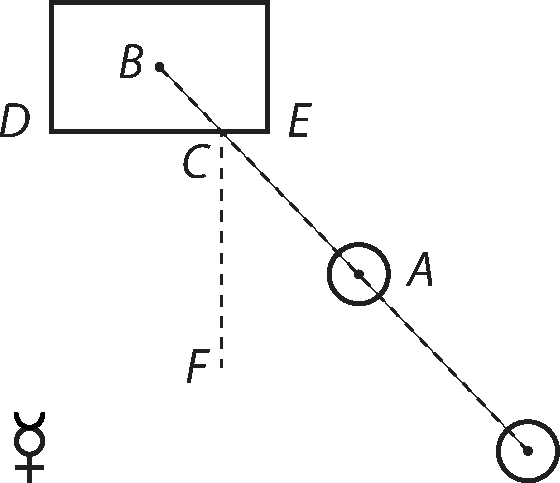
\includegraphics[width=0.315\textwidth]{gesamttex/edit_VIII,3/images/LH_37_05_090-091_d3.pdf}}%
  \vspace{0.5em}
  \centerline{\lbrack\textit{Fig.~3}\rbrack}%
  \label{LH_37_05_090v_Fig.3}%
  \vspace{1.5em}
\pstart%
%.   %.   %.   %.   ACHTUNG GETRIXT.   %.   %.   %.   %
\edtext{}{%
\lemma{\hspace{1,6mm}\lbrack\textit{Fig.~3}\rbrack}\killnumber\Cfootnote{%
Ein Entwurf hierzu wird nicht wiedergegeben.\hspace{15mm}}}%
\edtext{Si}{%
\lemma{Si corpus \textit{A}}\Cfootnote{%
Siehe \lbrack\textit{Fig.~3}\rbrack.}}
%
\edtext{corpus \textit{A} incurrat
in corpus quiescens \textit{B},%
\protect\index{Sachverzeichnis}{corpus incurrens in quiescens}%
\protect\index{Sachverzeichnis}{corpus quiescens}
ita ut linea motus \textit{AC} sit obliqua%
\protect\index{Sachverzeichnis}{linea motus obliqua}
ad lineam contactus \textit{DE},%
\protect\index{Sachverzeichnis}{linea contactus}%
}{%
\lemma{corpus \textit{A}}\Bfootnote{\hspace{-0,5mm}%
\textit{(1)}~oblique
\textit{(2)}~incurrat in \lbrack...\rbrack\ contactus \textit{DE},%
~\textit{L}}}
%
directe autem tendat in centrum \textit{B},
quaeritur
quis futurus sit eventus.%
\protect\index{Sachverzeichnis}{eventus futurus}
Hinc veras reflexionum regulas discemus%
\protect\index{Sachverzeichnis}{regulae reflexionum}
nec figmento de compositione motus fidemus.%
\protect\index{Sachverzeichnis}{figmentum de compositione motus}%
\protect\index{Sachverzeichnis}{compositio motus}
Et ut discamus
quid fiat
si corpus impingat in aliud immobile,%
\protect\index{Sachverzeichnis}{corpus impingens in immobile}%
\protect\index{Sachverzeichnis}{corpus immobile}
tunc ponamus ipsum excipiens \textit{B}
ponderis infiniti.%
\protect\index{Sachverzeichnis}{corpus excipiens ponderis infiniti}%
\protect\index{Sachverzeichnis}{pondus infinitum}
Verum tunc nihil discemus.%
\pend%
\pstart%
Ut rem distincte explicemus,
ab incursu puncti in punctum%
\protect\index{Sachverzeichnis}{incursus puncti in punctum}%
\protect\index{Sachverzeichnis}{punctum in punctum incurrens}
transeamus
%
\edtext{\lbrack ad\rbrack}{%
\lemma{ab}\Bfootnote{%
\textit{L~ändert Hrsg.}}}
%
incursum lineae in lineam.%
\protect\index{Sachverzeichnis}{incursus lineae in lineam}%
\protect\index{Sachverzeichnis}{linea in lineam incurrens}
Ubi quo tollantur difficultates,%
\protect\index{Sachverzeichnis}{difficultas}
sic rem concipiemus.
Esse corpus \textit{B} sine comparatione longius quam latius,%
\protect\index{Sachverzeichnis}{corpus sine comparatione longius quam latius}
ita ut latitudo haberi possit pro nulla
adeoque corpus poterit haberi pro linea,%
\protect\index{Sachverzeichnis}{corpus pro linea habitum}
et centrum gravitatis \textit{B} considerari
ut in corporis superficie positum.%
\protect\index{Sachverzeichnis}{centrum gravitatis in superficie positum}
Quod necesse est fingere,
ut scilicet
%
\edtext{simul non solum linea}{%
\lemma{simul}\Bfootnote{%
\textit{(1)}~utraque linea
\textit{(2)}~non solum linea%
~\textit{L}}}
%
motus obliqui,%
\protect\index{Sachverzeichnis}{linea motus}%
\protect\index{Sachverzeichnis}{motus obliquus}
sed et motus perpendicularis%
\protect\index{Sachverzeichnis}{motus perpendicularis}
quem continet
obliquus%
\protect\index{Sachverzeichnis}{motus obliquus}
%
\edtext{in centrum}{%
\lemma{in}\Bfootnote{%
\textit{(1)}~perpendicularem
\textit{(2)}~centrum%
~\textit{L}}}
%
gravitatis%
\protect\index{Sachverzeichnis}{centrum gravitatis corporis}
tendere intelligi possit,
quod effici non potest
si corpus crassitiem habeat,%
\protect\index{Sachverzeichnis}{corpus crassitiem habens}
ut in
%
\edtext{figura%
\protect\index{Sachverzeichnis}{figura}
signi \mercury.%
\protect\index{Sachverzeichnis}{signum mercurii}%
\protect\index{Sachverzeichnis}{mercurius}%
}{%
\lemma{figura signi \mercury\,}\Cfootnote{%
\lbrack\textit{Fig.~3}\rbrack.%
}}
%
\textit{AC} linea motus%
\protect\index{Sachverzeichnis}{linea motus}
tendit quidem in \textit{B},
centrum gravitatis corporis,
sed \textit{FC} perpendicularis ad \textit{DE},
in centrum gravitatis \textit{B}%
\protect\index{Sachverzeichnis}{centrum gravitatis corporis}
continuata
non tendit.%
\pend%
%
\pstart%
Caeterum
ut linea hoc modo in lineam moveri possit,%
\protect\index{Sachverzeichnis}{linea in lineam mota}
%
fingemus
\edtext{in
\edtext{fig.~$\astrosun$%
\protect\index{Sachverzeichnis}{figura solis}%
\protect\index{Sachverzeichnis}{sol}%
}{%
\lemma{fig.~$\astrosun$}\Cfootnote{%
\lbrack\textit{Fig.~4}\rbrack\
auf S.~\pageref{LH_37_05_090v_Fig.4}.}}%
}{%
\lemma{in}\Bfootnote{%
\hspace{-0,5mm}fig.~$\astrosun$
\textit{erg.~L}}}
%
lineam
cujus centrum gravitatis \textit{A} esse in alio plano,%
\protect\index{Sachverzeichnis}{centrum gravitatis lineae}
et hoc planum tantum secare in puncto \textit{A},
atque ita
%
\edtext{incurrere in lineam quiescentem majorem%
\protect\index{Sachverzeichnis}{incursus lineae in lineam}%
}{%
\lemma{incurrere}\Bfootnote{%
\hspace{-0,5mm}in
\textit{(1)}~corpus quiescens majus
\textit{(2)}~lineam quiescentem majorem%
~\textit{L}}}
%
se,
nempe \textit{B}.
Certum est nonnihil \makebox[1.0\textwidth][s]{debere
%
\edtext{reflecti \textit{A},%
\protect\index{Sachverzeichnis}{linea reflexa}%
}{%
\lemma{reflecti}\Bfootnote{\hspace{-0,5mm}%
\textbar~corpus \textit{gestr.}~%
\textbar\ \textit{A},%
~\textit{L}}}
%
et \textit{B} pergere.%
\protect\index{Sachverzeichnis}{linea pergens}
Ponamus
centrum gravitatis utriusque lineae \textit{C}%
\protect\index{Sachverzeichnis}{centrum gravitatis lineae}
progredi}
\pend
\newpage
% Diagramm Fig.~4
  \centerline{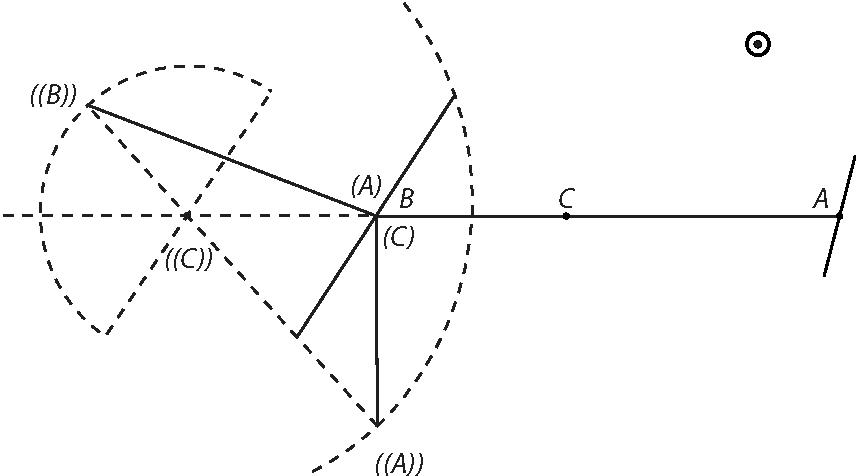
\includegraphics[width=0.8\textwidth]{gesamttex/edit_VIII,3/images/LH_37_05_090-091_d4.pdf}}%
  \vspace{0.5em}
  \centerline{\lbrack\textit{Fig.~4}\rbrack}%
  \label{LH_37_05_090v_Fig.4}%
  \vspace{1.5em}%
%
\pstart
\noindent in eadem recta,
quod utique indubium
%
\edtext{ex demonstratis}{%
\lemma{ex demonstratis}\Cfootnote{%
Der Beweis, dass beim zentralen Stoß zweier Körper die gleichförmige Geschwindigkeit und die Richtung des gemeinsamen Schwerpunkts erhalten bleiben, erfolgte in 
N.~\ref{dcc_09}.% ??S01\textsubscript{11}.%
}}%
\lbrack,\rbrack\
%
erit ergo primus ejus locus \textit{C},
secundus \textit{(C)} coincidens cum
%
\edtext{\textit{(A)} et \textit{B},}{%
\lemma{\textit{Am Rand:}}\Afootnote{%
\textit{(B)} et \textit{B} idem hic in casu quietis \textit{B}.%
\protect\index{Sachverzeichnis}{quies}%
\protect\index{Sachverzeichnis}{casus quietis}%
}}
%
tertius
%
\edtext{\lbrack\textit{((C))}\rbrack}{%
\lemma{\textit{((C))(C)}}\Bfootnote{%
\textit{L~ändert Hrsg. nach~E, S.~169}%
\cite{01056}}}
%
et erit \textit{((C))(C)} aequ. \textit{(C)C},
necesse est
%
\edtext{autem tria puncta}{%
\lemma{autem}\Bfootnote{%
\textit{(1)}~corpora
\textit{(2)}~tria puncta%
~\textit{L}}}
%
\textit{((B))}, \textit{((C))} et \textit{((A))}
esse in eadem recta,
et \textit{((B))((C))} esse ad \textit{((A))((C))}
ut \textit{BC} ad \textit{AC},
id est in reciproca corporum;
quod si eadem
ante et post concursum
deberet corporum \textit{B},
\textit{A} distantia esse,%
\protect\index{Sachverzeichnis}{distantia corporum concurrentium}
forent rectae \textit{((A))((C))} et \textit{((C))((B))} et \textit{((A))((B))} datae,
aequales \textit{AC}, \textit{CB}, \textit{AB}.
Hinc jam rectae
%
\edtext{\lbrack\textit{B((B))}\rbrack}{%
\lemma{\textit{(B)B}}\Bfootnote{%
\textit{L~ändert Hrsg.}}}
%
et \textit{(A)((A))} debent esse tales,
ut quadratum illius in corpus \textit{B}
junctum quadrato hujus in corpus \textit{A},
aequatur quadrato \textit{A(A)} in corpus \textit{A}.
Ubi si ponamus \textit{((A))((B))} aequ. \textit{AB},
seu corporum distantiam manere eandem,%
\protect\index{Sachverzeichnis}{distantia corporum concurrentium}
et hanc
quam dixi
ponendo summam quadratorum celeritatum in corpora ductorum,%
\protect\index{Sachverzeichnis}{quadratum celeritatis ductum in corpus}
videndum
an possit esse \textit{((B))((A))} perpendicularis ad corpus \textit{B}.
Sed \makebox[1.0\textwidth][s]{quia nondum in calculum intravit%
\protect\index{Sachverzeichnis}{calculus}
rectane esset an curva linea, etc.,%
\protect\index{Sachverzeichnis}{linea recta}%
\protect\index{Sachverzeichnis}{linea curva}
ideo dubito
an ex}
\pend
\newpage
\pstart
\noindent solis illis datis%
\protect\index{Sachverzeichnis}{datum}
res queat determinari.
%
\edtext{Nota%
\lbrack:\rbrack\
ponenda linea}{%
\lemma{Nota}\Bfootnote{%
\textit{(1)}~ponendum corpus
\textit{(2)}~ponenda linea%
~\textit{L}}}
%
recta \textit{A} perpendicularis ad rectam \textit{AB},
alioqui rursus alia oriretur variatio%
\protect\index{Sachverzeichnis}{variatio}
ob duplicem obliquitatem.%
\protect\index{Sachverzeichnis}{obliquitas duplex}%
%
\edtext{}{%
\lemma{\textit{Am Ende des Absatzes:}}\Afootnote{%
\textls{Mira res}%
\protect\index{Sachverzeichnis}{res mira}}}
%
\lbrack91~v\textsuperscript{o}\rbrack\ %%%%    Blatt 91v
%
\pend%
 \pstart%
Compositionis motuum arcanum tandem inveni:%
\protect\index{Sachverzeichnis}{compositio motus}%
\protect\index{Sachverzeichnis}{arcanum compositionis motuum}
sint
%
\edtext{duo globi%
\protect\index{Sachverzeichnis}{globus in globos incurrens}
\textit{B}, \textit{D}
aequales inter se,
et cum tertio \textit{A},
qui}{%
\lemma{duo}\Bfootnote{%
\textit{(1)}~corpora
\textit{(2)}~globi \textit{B}, \textit{D}
\textit{(a)}~aequalia
\textit{(b)}~ejusdem
\textit{(c)}~aequales inter % se, et cum 
\lbrack...\rbrack\ tertio \textit{A},
\textbar~et
\textit{(1)}~ejusdem
\textit{(2)}~\textlangle omnes \textendash\textrangle\
\textit{erg. u. gestr.}~\textbar\
\textit{(aa)}~quod
\textit{(bb)}~qui%
~\textit{L}}}
%
ita in eos incurrit,%
\protect\index{Sachverzeichnis}{incursus globi in globos}
%
\edtext{ut tres globi}{%
\lemma{ut}\Bfootnote{%
\textit{(1)}~tria corpora
\textit{(2)}~tres globi%
~\textit{L}}}
%
\textit{(A)}, \textit{B}, \textit{D}
constituant angulum rectum,%
\protect\index{Sachverzeichnis}{angulus incursus rectus}
et uno adhuc latu accedente,
complerent
%
\edtext{quadratum angulos in eorum centris habens,
cujus quadrati diagonalem%
\protect\index{Sachverzeichnis}{diagonalis quadrati}%
}{%
\lemma{quadratum}\Bfootnote{%
\textit{(1)}~, cujus quadrata diagona
\textit{(2)}~angulos in % eorum centris habens, cujus 
\lbrack...\rbrack\ quadrati diagonalem%
~\textit{L}}}
%
faciat producta \textit{A(A)};
%
\edtext{patet
si globum \textit{A}%
\protect\index{Sachverzeichnis}{globus in globos incurrens}
quasi}{%
\lemma{patet}\Bfootnote{%
\textit{(1)}~si corpus \textit{A} qua
\textit{(2)}~si globum \textit{A} quasi%
~\textit{L}}}
%
duobus motibus venisse
ponamus,
uno \textit{E(A)},
altero \textit{F(A)},
posito \textit{A(A)} esse diagonalem quadrati \textit{FE},%
\protect\index{Sachverzeichnis}{diagonalis quadrati}
ipsum uno quidem motu propulsurum corpus \textit{D} in \textit{((D))}
celeritate \textit{D((D))} aequ. \textit{E(A)},%
\protect\index{Sachverzeichnis}{celeritas propulsionis}
altero corpus \textit{B} in \textit{((B))}
celeritate \textit{B((B))} aequ. \textit{F(A)},%
\protect\index{Sachverzeichnis}{celeritas propulsionis}
%
\edtext{ipsum autem ob aequalitatem%
\protect\index{Sachverzeichnis}{aequalitas corporum concurrentium}
amittet suum%
\protect\index{Sachverzeichnis}{motus corporis propellentis}
et quiescet in loco \textit{A},%
\protect\index{Sachverzeichnis}{corpus quiescens}%
}{%
\lemma{ipsum}\Bfootnote{%
\hspace{-0,5mm}autem % ob aequalitatem amittet suum et quiescet in 
\lbrack...\rbrack\ loco \textit{A},
\textit{erg.~L}}}
%
unde
\edtext{augetur motus.%
\protect\index{Sachverzeichnis}{motus auctus}%
}{%
\lemma{augetur}\Bfootnote{%
\textit{(1)}~quantitas
\textit{(2)}~motus.%
~\textit{L}}}
%
Quis enim non videt ob aequalitatem corporum,%
\protect\index{Sachverzeichnis}{aequalitas corporum concurrentium}
quantitatem motus%
\protect\index{Sachverzeichnis}{quantitas motus corporum concurrentium}
%
\edtext{quae erit}{%
\lemma{quae}\Bfootnote{%
\textit{(1)}~fuit
\textit{(2)}~erit~%
\textit{L}}}
%
post ictum,%
\protect\index{Sachverzeichnis}{ictus}
majorem esse quam
%
\edtext{quae fuit}{%
\lemma{quae}\Bfootnote{%
\textit{(1)}~erit
\textit{(2)}~fuit%
~\textit{L}}}
%
ante ictum,%
\protect\index{Sachverzeichnis}{ictus}
%
\edtext{nempe ut latus duplicatum}{%
\lemma{nempe ut}\Bfootnote{%
\textit{(1)}~summa
\textit{(2)}~latus%
~\textit{L}}}
%
quadrati%
\protect\index{Sachverzeichnis}{latus quadrati duplicatum}
ad diagonalem.%
\protect\index{Sachverzeichnis}{diagonalis quadrati}
%
\edtext{Verum mirifice evenit,
ut}{%
\lemma{Verum}\Bfootnote{%
\textit{(1)}~quod
\textit{(2)}~mirifice evenit, ut%
~\textit{L}}}
%
nihilominus eaedem maneant vires,%
\protect\index{Sachverzeichnis}{vis eadem manens}
\hspace{0.1mm}quia
%
\hspace{0.1mm}\edtext{eadem \hspace{0.1mm}manent \hspace{0.1mm}quadrata}{%
\lemma{eadem}\Bfootnote{%
\textit{(1)}~manebit
\textit{(2)}~manent%
~\textit{L}}}
%
\hspace{0.1mm}celeritatum
\pend
 \vspace{1.5em}%	% Diagramm Fig.~5
  \centerline{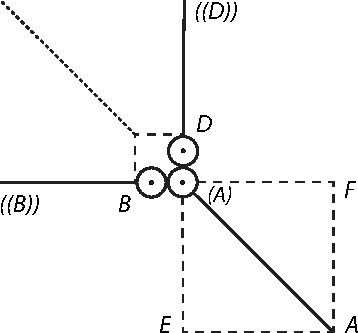
\includegraphics[width=0.395\textwidth]{gesamttex/edit_VIII,3/images/LH_37_05_090-091_d5.pdf}}%
  \vspace{0.5em}
  \centerline{\lbrack\textit{Fig.~5}\rbrack}%
%  \label{LH_37_05_091v_Fig.5}%
 %
\newpage
\pstart
\noindent in corpora%
\protect\index{Sachverzeichnis}{quadratum celeritatis ductum in corpus}
%
\edtext{ducta,
nam}{%
\lemma{ducta,}\Bfootnote{%
\textit{(1)}~id est
\textit{(2)}~nam%
~\textit{L}}}
%
quadratum a diagonali%
\protect\index{Sachverzeichnis}{quadratum a diagonali}
aequale quadratis duorum laterum%
\protect\index{Sachverzeichnis}{quadrata duorum laterum conjugatorum}
simul sumptis.
Hinc etsi
%
\edtext{\textit{A(A)} linea}{%
\lemma{\textit{A(A)}}\Bfootnote{%
\textit{(1)}~recta
\textit{(2)}~linea%
~\textit{L}}}
%
motus%
\protect\index{Sachverzeichnis}{linea motus}
non fuisset diagonius quadrati \textit{D(A)B},%
\protect\index{Sachverzeichnis}{diagonius quadrati}
tamen res successisset
quamquam alia ratione%
\lbrack:\rbrack\
quia in omni parallelogrammo rectangulo%
\protect\index{Sachverzeichnis}{parallelogrammum rectangulum}
summa a quadratis duorum laterum conjugatorum%
\protect\index{Sachverzeichnis}{quadrata duorum laterum conjugatorum}
aequalis quadrato diagonii.%
\protect\index{Sachverzeichnis}{quadratum diagonii}
Ideo in omni proposita fingi potest,
salvis viribus,%
\protect\index{Sachverzeichnis}{vis salva}
corpus
%
\edtext{ferri
\lbrack motu\rbrack\
rectanguli%
\protect\index{Sachverzeichnis}{motus rectanguli}%
}{%
\lemma{ferri}\Bfootnote{%
\textit{(1)}~motu dia
\textit{(2)}~\textbar~motu \textit{erg. Hrsg. nach~E, S.~171\cite{01056}}
\textit{(a)}~parallelogrammi
\textit{(b)}~rectanguli%
~\textit{L}}}
%
cujuslibet,
cujus diagonium sit recta data.%
\protect\index{Sachverzeichnis}{diagonium rectanguli}
\pend%
%
\pstart%
%%
%%
%%
%%
%%\noindent\begin{wrapfigure}{l}{0.6\textwidth}
%\vspace*{1em}
%\begin{minipage}[t]{0.4\textwidth}
%\hspace*{-5mm}
%\includegraphics[width=1\textwidth]{gesamttex/edit_VIII,3/images/lh37,5,91v-2.pdf}
%\noindent \centering [\textit{Fig.~2}]
%\vspace*{1ex}
%\end{minipage}
%\hspace*{7,3mm}
%\begin{minipage}[t]{0.5\textwidth}
%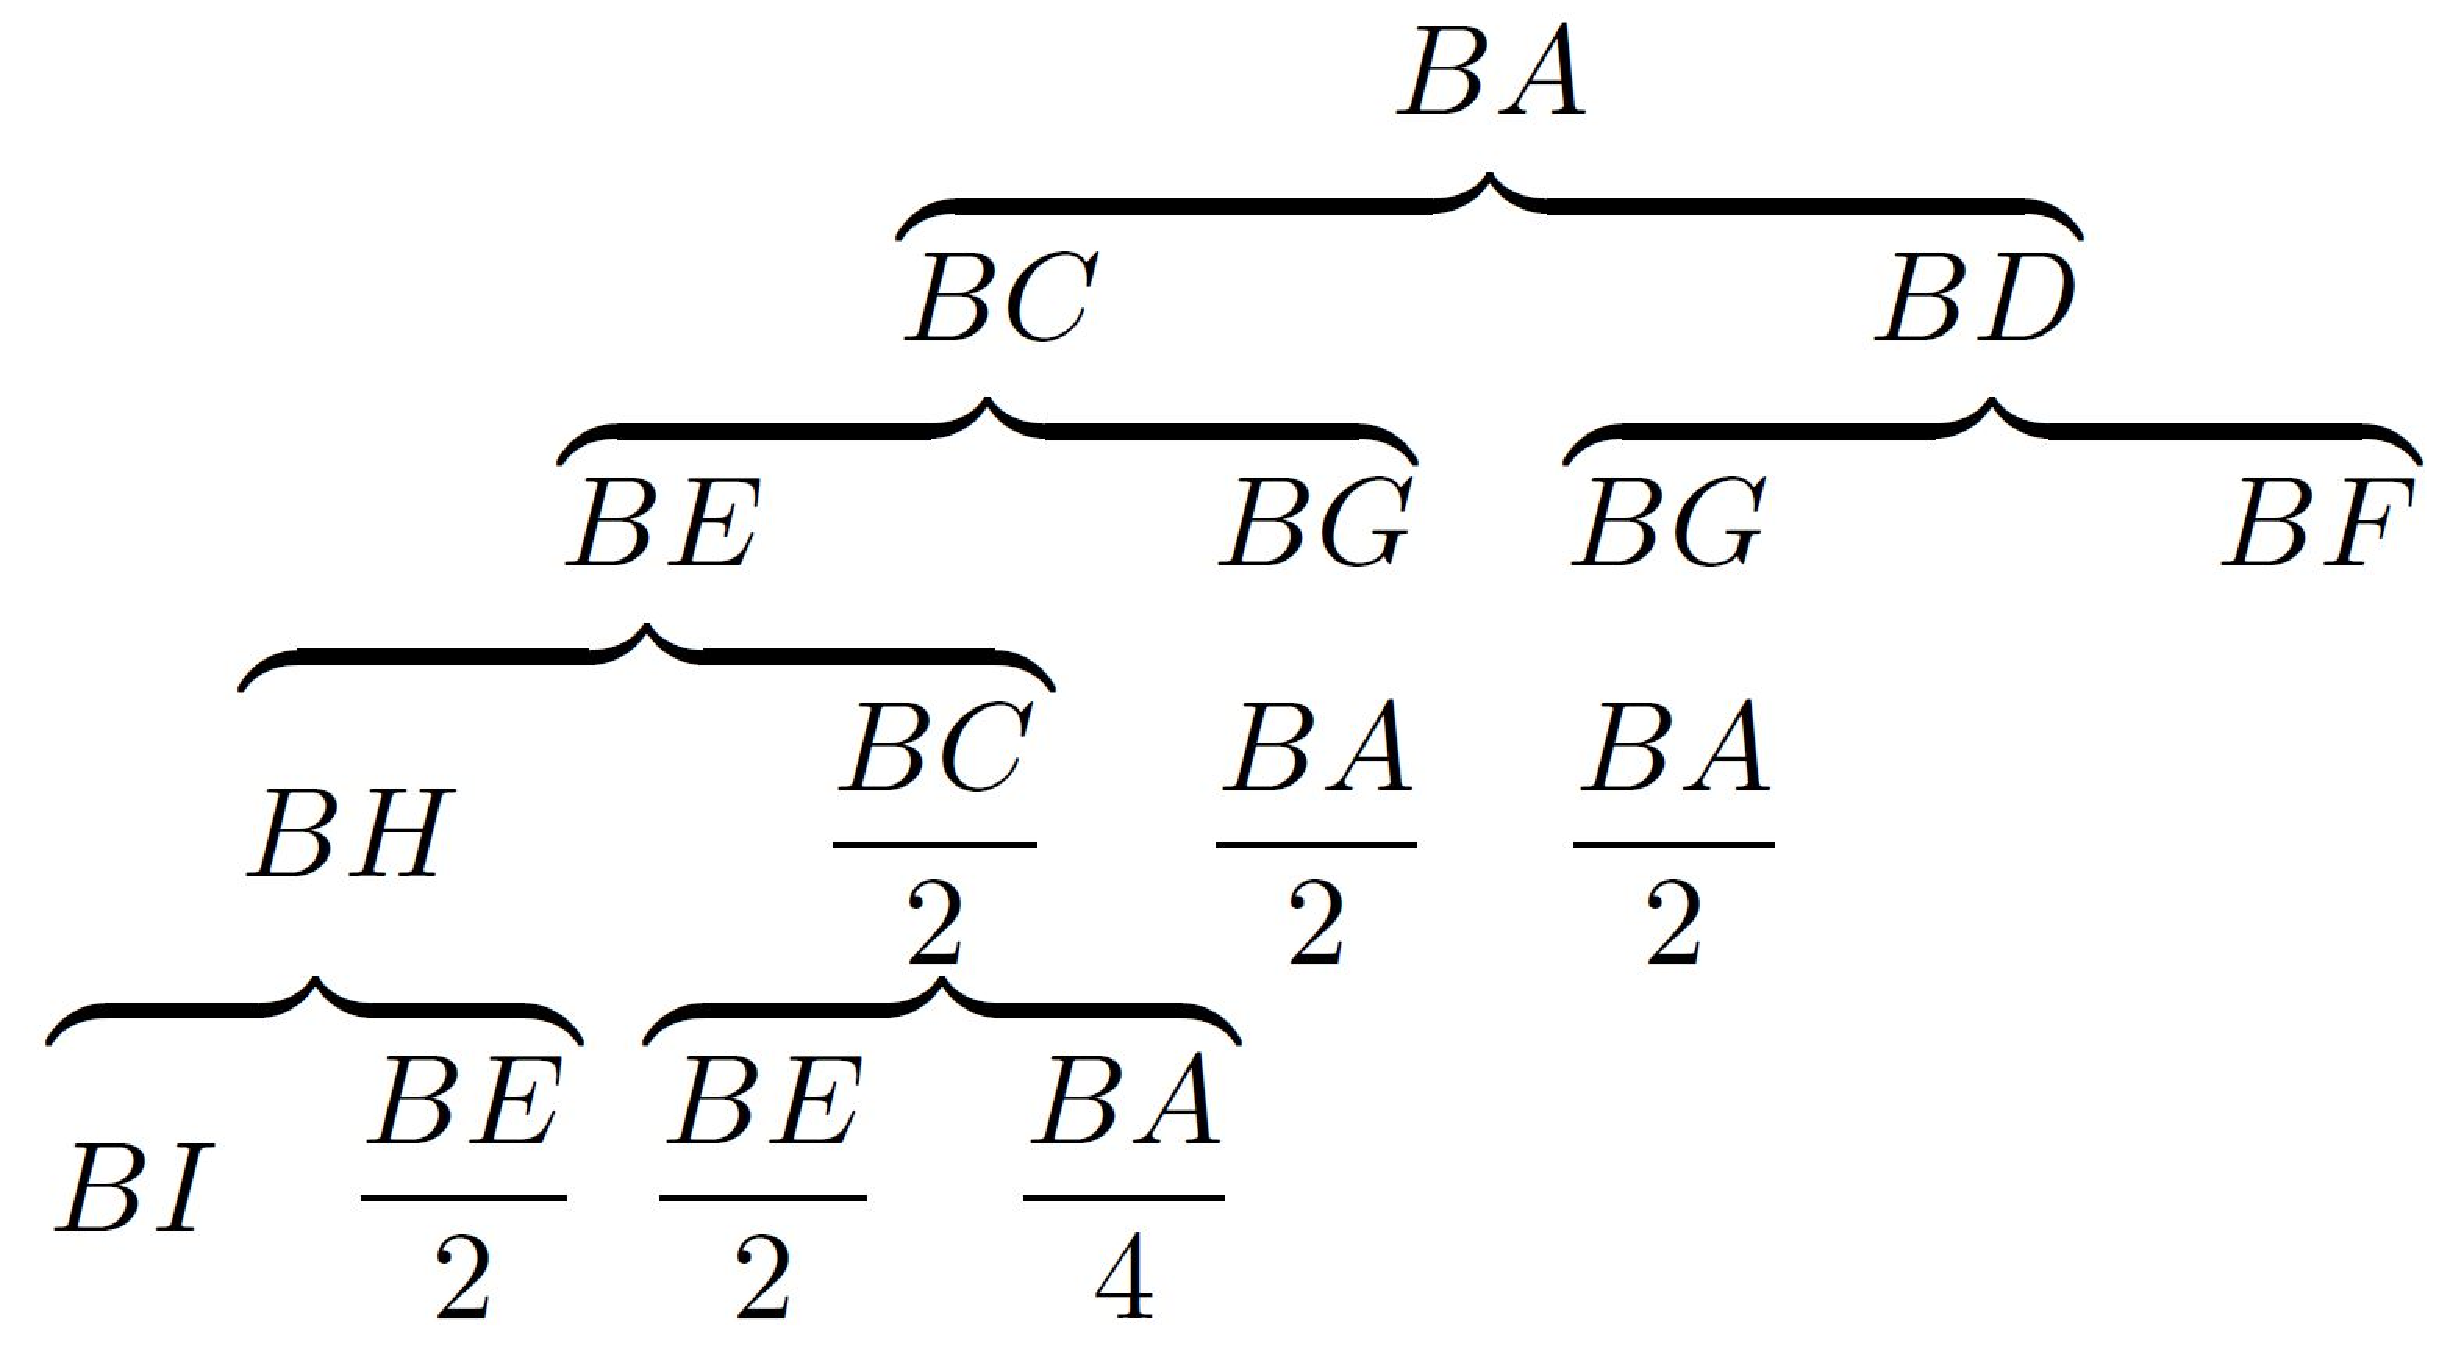
\includegraphics[width=1\textwidth]{gesamttex/edit_VIII,3/images/overbrace-test.pdf}
%%\begin{minipage}[t]{120pt}
%%$\begin{array}{c}
%%\hspace{40pt} BA\\
%%\hspace{40pt} \overbrace{BC \hspace{60pt} BD}\\
%%\hspace{40pt} \overbrace{BE \hspace{35pt} BG} \hspace{10pt} \overbrace{BG \hspace{35pt} BF}\\
%%\protect \makebox[15pt]{} \overbrace{BH \hspace{28pt} \displaystyle\frac{BC}{2}} \hspace{10pt} \displaystyle\frac{BA}{2}\hspace{10pt} \displaystyle\frac{BA}{2} \hfill\\
%%\overbrace{BI \hspace{10pt} \displaystyle\frac{BE}{2}} \ \overbrace{\displaystyle\frac{BE}{2} \hspace{10pt} \displaystyle\frac{BA}{4}} \hfill
%%\end{array}$
%\end{minipage}
%%\end{wrapfigure}
%\pend \pstart
%%
%%
%%
%%
Hinc mirifica elici potest speculatio:%
\protect\index{Sachverzeichnis}{speculatio mirifica}
si quamlibet rectam
quae latus%
\protect\index{Sachverzeichnis}{latus rectanguli}
%
\edtext{est unius rectanguli,
rursus diagonion facias alterius rectanguli%
\protect\index{Sachverzeichnis}{diagonium rectanguli}%
}{%
\lemma{est}\Bfootnote{%
\textit{(1)}~parallel
\textit{(2)}~ad
\textit{(3)}~rursus alterius
\textit{(4)}~unius rectanguli, % rursus diagonium facias 
\lbrack...\rbrack\ alterius rectanguli%
~\textit{L}}}
%
et
%
\edtext{ita porro,
illis tantum exceptis
\lbrack\textit{Satz bricht ab.}\rbrack\
Determinatum est autem
quae sit ratio \textit{BL}
(\protect\vphantom)%
quae in ipsam \textit{BA},
sed contrario conatu%
\protect\index{Sachverzeichnis}{conatus contrarius}
rursus incidit%
\protect\vphantom()
ad ipsam \textit{BA}.
Ergo determinavimus conatus%
\protect\index{Sachverzeichnis}{conatus compositus}
in aliqua recta,
ex quibus momentis prorsum et retrorsum%
\protect\index{Sachverzeichnis}{momentum prorsum et retrorsum}
in eadem recta compositus%
\protect\index{Sachverzeichnis}{conatus compositus}
intelligi possit
salvis viribus.%
\protect\index{Sachverzeichnis}{vis salva}%
}{%
\lemma{ita}\Bfootnote{%
\textit{(1)}~in infinitum,
\textit{(2)}~porro, illis tantum exceptis \lbrack\textit{Satz bricht ab.}\rbrack\
\textit{(a)}~Sed hinc facile colligi potest considerandum esse rectangulum aequilaterum \textit{ABM}, et fingendum quasi corpus tenderet a \textit{B} versus \textit{A} celeritate%
\protect\index{Sachverzeichnis}{rectangulum aequilaterum}%
\protect\index{Sachverzeichnis}{corpus tendens}
\textit{(aa)}~\textit{BM}
\textit{(bb)}~\textit{AM}
\textit{(cc)}~\textit{MA}, et retrorsum tenderet.
\textit{(b)}~Determinatum est % 
\lbrack...\rbrack\ Ergo determinavimus
\textit{(aa)}~quis sit
\textit{(bb)}~conatus in % aliqua recta, 
\lbrack...\rbrack\ ex quibus
\textit{(aaa)}~conatibus
\textit{(bbb)}~momentis prorsum et retrorsum
\textit{(aaaa)}~compositus intelligi possit
\textit{(bbbb)}~in eadem % recta compositus intelligi possit 
\lbrack...\rbrack\ salvis viribus.%
~\textit{L}}}
%
Quae valde paradoxa inquisitio est.%
\protect\index{Sachverzeichnis}{inquisitio paradoxa}
Sed tunc etiam patet,
quasvis alias motus compositiones%
\protect\index{Sachverzeichnis}{compositio motus}
salvis viribus%
\protect\index{Sachverzeichnis}{vis salva}
non posse admitti,
nisi reapse duplices impulsus deprehendantur.%
\protect\index{Sachverzeichnis}{impulsus duplex}%
%.   %.   %.   %.   Achtung getrixt.   %.   %.   %.   %.
%
\edtext{}{%
\lemma{\hspace{1,6mm}\lbrack\textit{Fig.~6}\rbrack}\killnumber\Cfootnote{%
Das Dreieck \textit{BLH} hat Leibniz schließlich gestrichen.}}
\pend%
%
%
%  \newpage% 
  \vspace{1.2em}%	% Diagramm Fig.~6
  \centerline{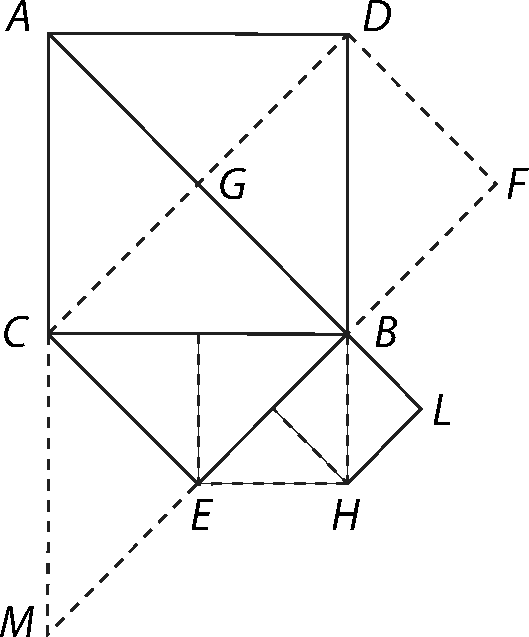
\includegraphics[width=0.32\textwidth]{gesamttex/edit_VIII,3/images/LH_37_05_090-091_d6.pdf}}%
  \vspace{0.3em}
  \centerline{\lbrack\textit{Fig.~6}\rbrack}%
%  \vspace{-15.0em}%
%  \centerline{\hspace{65mm}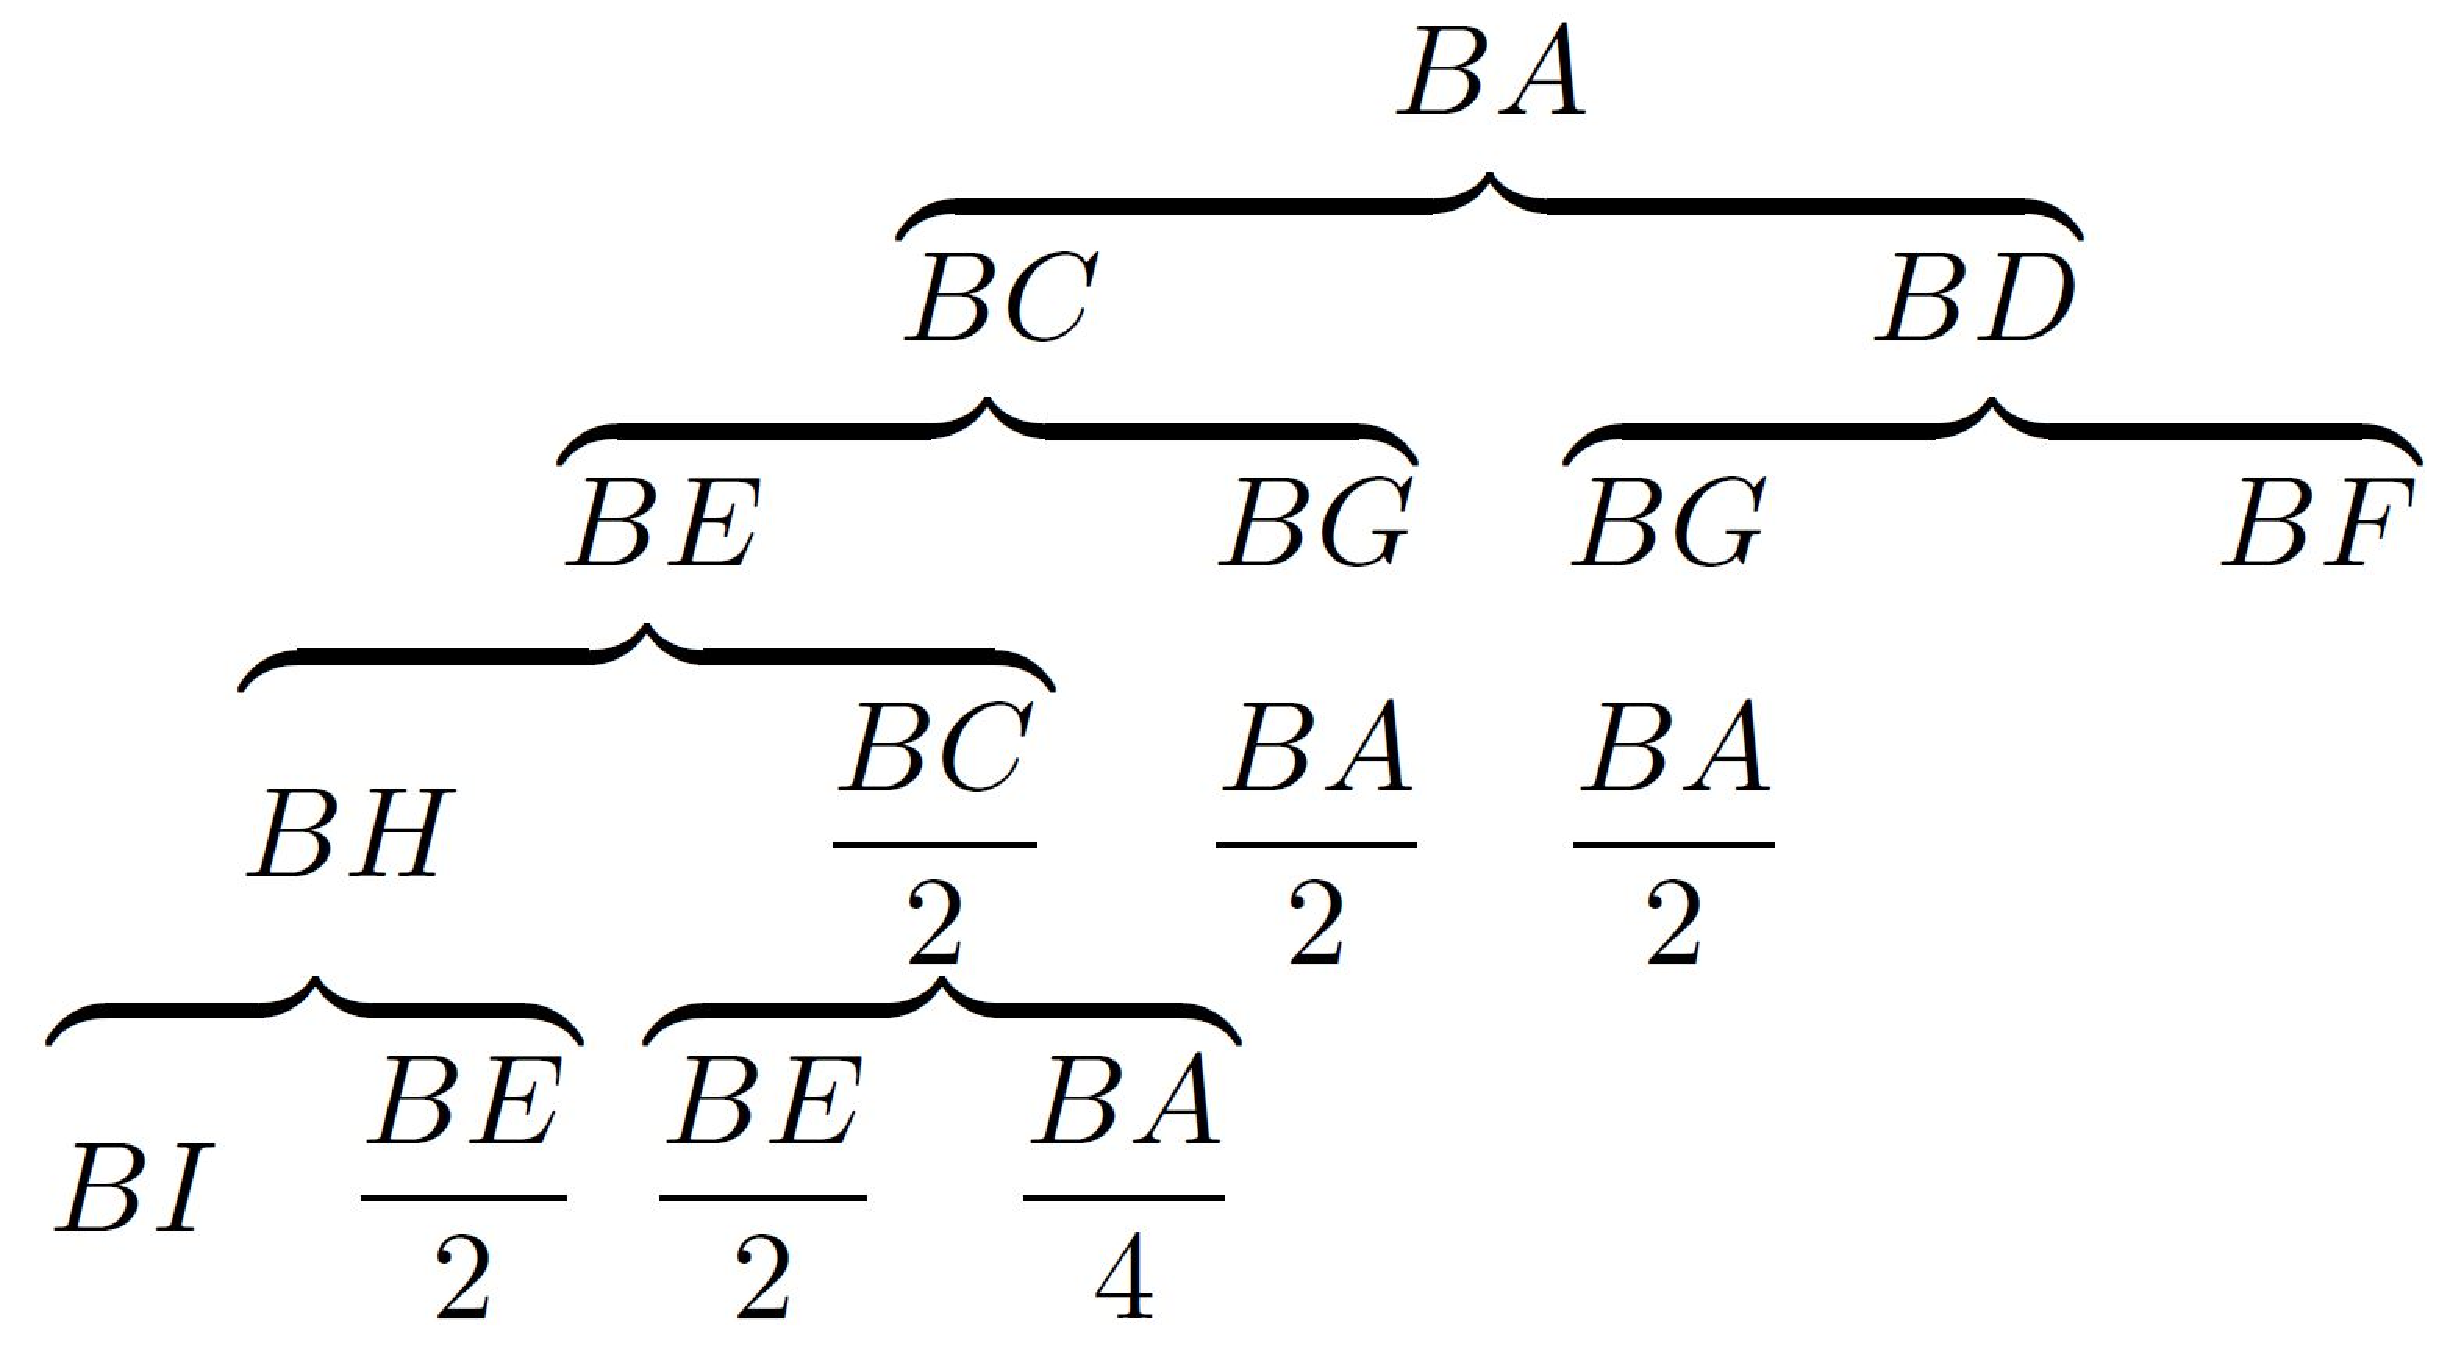
\includegraphics[width=0.44\textwidth]{gesamttex/edit_VIII,3/images/overbrace-test.pdf}}%
%  \label{LH_37_05_091v_Fig.6}%
%  \vspace{1.5em}%
%
\pstart%
\noindent%
\lbrack\textit{Neben dem Diagramm:}\rbrack\ % \textit{Fig.~6}
\newline%
\newline%
$
%%%%% 1
\hspace*{40mm}%
BA
\newline%
%%%%% 2
\hspace*{24,5mm}%
\overbrace{%
\displaystyle BC
\hspace*{23,5mm}%
\displaystyle BD}^{\displaystyle }%
\newline%
%%%%% 3
\hspace*{14mm}%
\overbrace{%
BE
\hspace*{15mm}%
\displaystyle BG}^{\displaystyle }
\hspace*{5mm}%
\overbrace{%
BG
\hspace*{10mm}%
\displaystyle BF}^{\displaystyle }%
\newline%
%%%%% 4
\hspace*{5mm}%
\overbrace{%
\displaystyle BH \hspace{11mm} \displaystyle \frac{BC}{2}}^{\displaystyle }
\hspace{5,25mm}%
\displaystyle \frac{BA}{2}
\hspace{5,5mm}%
\displaystyle \frac{BA}{2}
\newline%
%%%%% 5
\overbrace{%
\displaystyle [BL] \ \displaystyle \frac{BE}{2}}^{\displaystyle }
\ \ \,
\overbrace{%
\displaystyle \frac{BE}{2} \ \displaystyle \frac{BA}{4}}^{\displaystyle }%
\edtext{}{\lemma{$-\,BL$}\Bfootnote{\textit{L~ändert Hrsg.}}}
\newline%
%%%%% 6
\overbrace{%
\phantom{\displaystyle [BL] \ }%
}^{}%
$
\pend%
\count\Bfootins=1200%
\count\Afootins=1200%
\count\Cfootins=1200
%
%
%%%%    Ende des Textes auf Blatt 91v.  BH \ \frac{BC}{2}
%
%